\documentclass[tikz]{standalone}
\usepackage{pgfplots}
\pgfplotsset{compat=1.18}
\usepackage{pgfplotstable}

\begin{document}
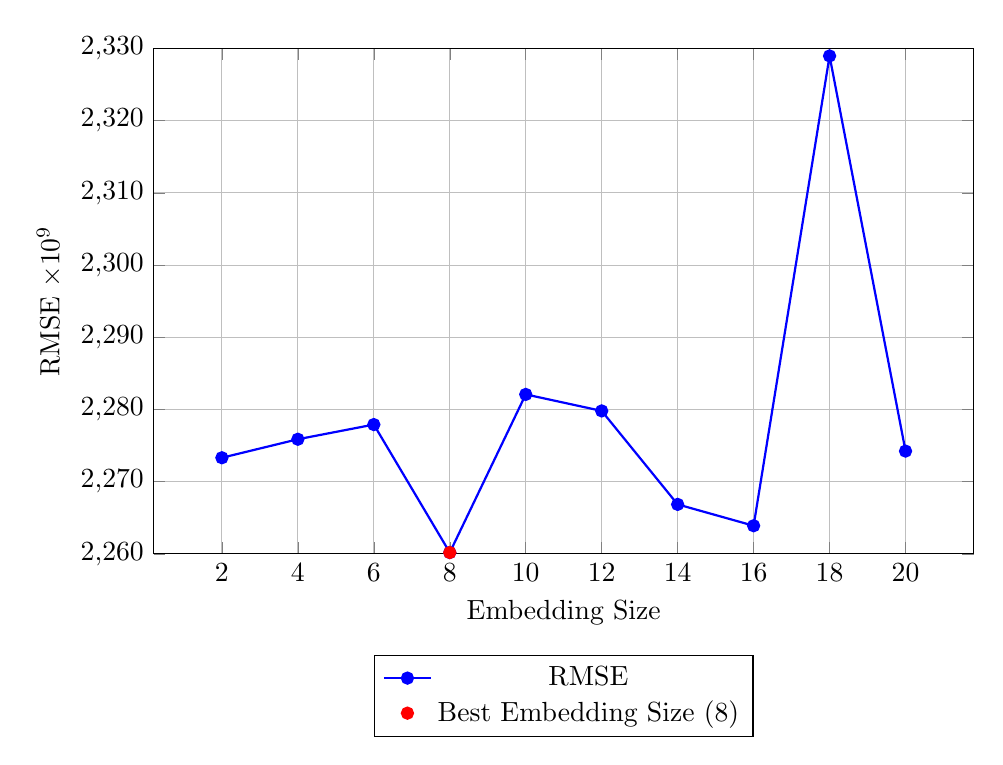
\begin{tikzpicture}
\begin{axis}[
    width=12cm,
    height=8cm,
    xlabel={Embedding Size},
    ylabel={RMSE $\times 10^9$},
    xtick={2,4,6,8,10,12,14,16,18,20},
    ymin=2260, ymax=2330,
    grid=both,
    ticklabel style={/pgf/number format/fixed},
    legend style={at={(0.5,-0.2)}, anchor=north, legend columns=1},
    ymajorgrids=true,
    xmajorgrids=true,
    every axis plot/.append style={thick}
]

% Data points
\addplot[blue, mark=*] coordinates {
    (2, 2273.3140356245127)
    (4, 2275.8780866363516)
    (6, 2277.911010240325)
    (8, 2260.187076623008)
    (10, 2282.0883218417397)
    (12, 2279.802522059339)
    (14, 2266.8541478489223)
    (16, 2263.8975346567087)
    (18, 2328.9712910762267)
    (20, 2274.238255887034)
};

% Highlight the best embedding size
\addplot[red, only marks, mark=*] coordinates {
    (8, 2260.187076623008)
};

\legend{RMSE, Best Embedding Size (8)}

\end{axis}
\end{tikzpicture}

\end{document}
